\section{Fractals}

% FRAME 14
\begin{frame}{Fractals}
	\begin{figure}
		\centering
		\includegraphics[width = 8cm]{Pictures/fractalcover.jpg}
		\caption{Fractal (\cite{fractalcover})}
		\label{fig:enter-label}
	\end{figure}
	
\end{frame}

% FRAME 15
\begin{frame}{Motivation}
	\begin{itemize}
		\item Coastline
		\item Lungs
		\begin{figure}
			\centering
			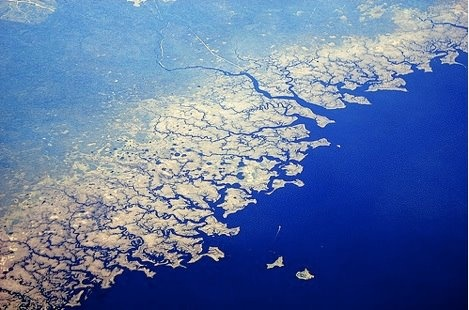
\includegraphics[width = 5cm]{Pictures/coastline.jpg}
			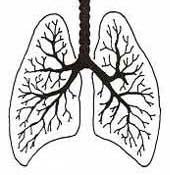
\includegraphics[height = 3.4cm, width  = 4cm]{Pictures/lungs.jpg}
			\caption{Coastline and lung (\cite{COastline} and \cite{Lung})}
			\label{fig:enter-label}
		\end{figure}
		
	\end{itemize}
\end{frame}



% FRAME 16
\begin{frame}{Motivation}
	\begin{itemize}
		\item 1872: Karl Weierstrass constructed a function that is continuous but nowhere differentiable:
		$$f(x) = \sum\limits_{n=0}^{\infty}a^ncos(b^n\pi x)$$
	\end{itemize}
	\begin{itemize}
		\item 1904: Helge von Koch devised a geometric method to construct pathological curves.
	\end{itemize}
	\begin{itemize}
		\item 1915: Wacław Sierpiński introduced Sierpiński triangle.
	\end{itemize}
	\begin{itemize}
		\item 1918: Gaston Julia & Pierre Fatou studied iteration of complex functions.
	\end{itemize}
\end{frame}


	\begin{frame}{Geometric Fractals}
		\begin{figure}
		\centering
			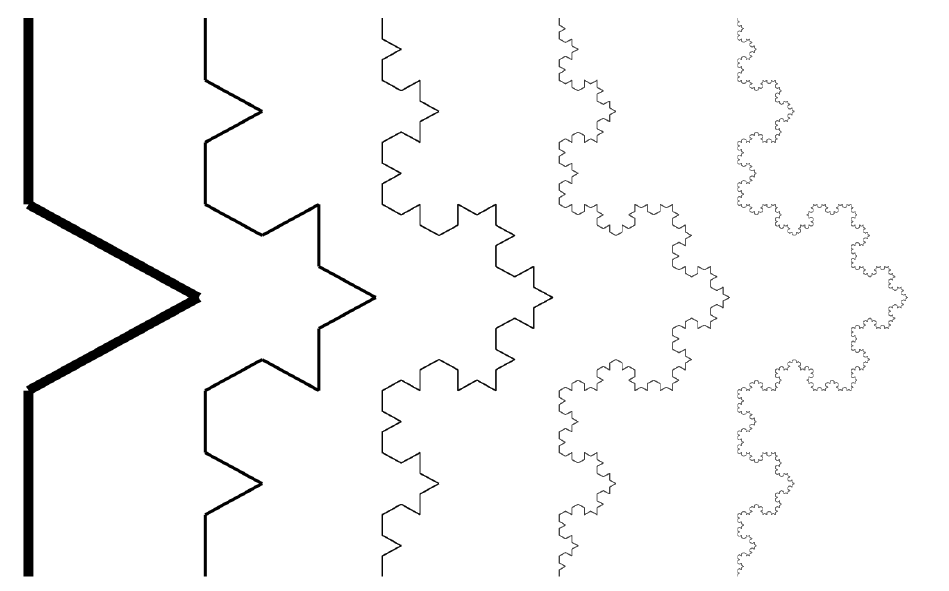
\includegraphics[width = 9cm, height = 5cm  ]{images/Koch1.png}
			\caption{Koch curve \space
			(\cite{frac})}
			\label{koch}
		\end{figure}
		\end{frame}
		\begin{frame}{Algebraic Fractals}
		\begin{figure}
			\centering
			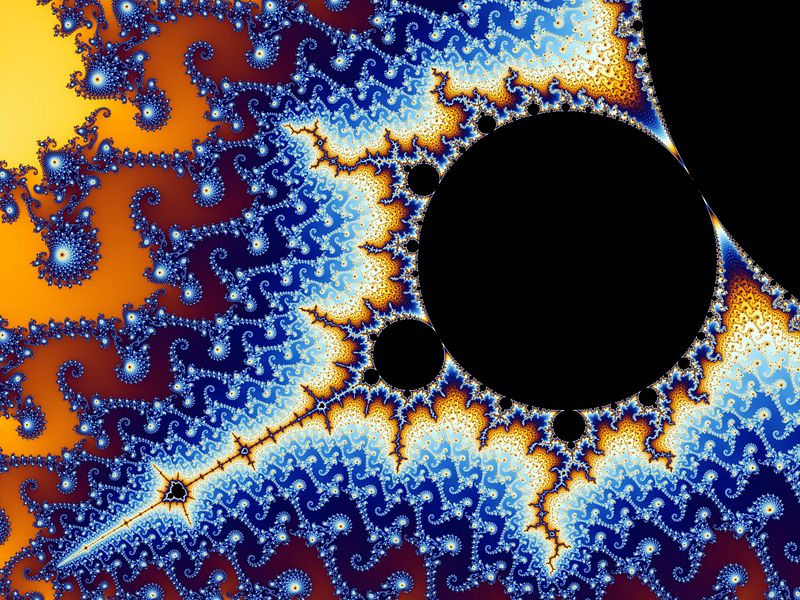
\includegraphics[width = 9cm, height = 5cm  ]{images/mandelbrot.jpg}
			\caption{Section of a Mandelbrot set \space
			(\cite{wiki:xxx})}
			\label{mandel}
		\end{figure}
		\end{frame}
		
\begin{frame}{Fractal Dimension}
	\begin{itemize}
		\item Key Question: How does the object scale?
	\end{itemize}
	\begin{figure}
		\centering
		\includegraphics[width=0.2\linewidth]{../../../../../../Desktop/Cube/signs-line-straight-minus-horizontal-png-icon-14}
		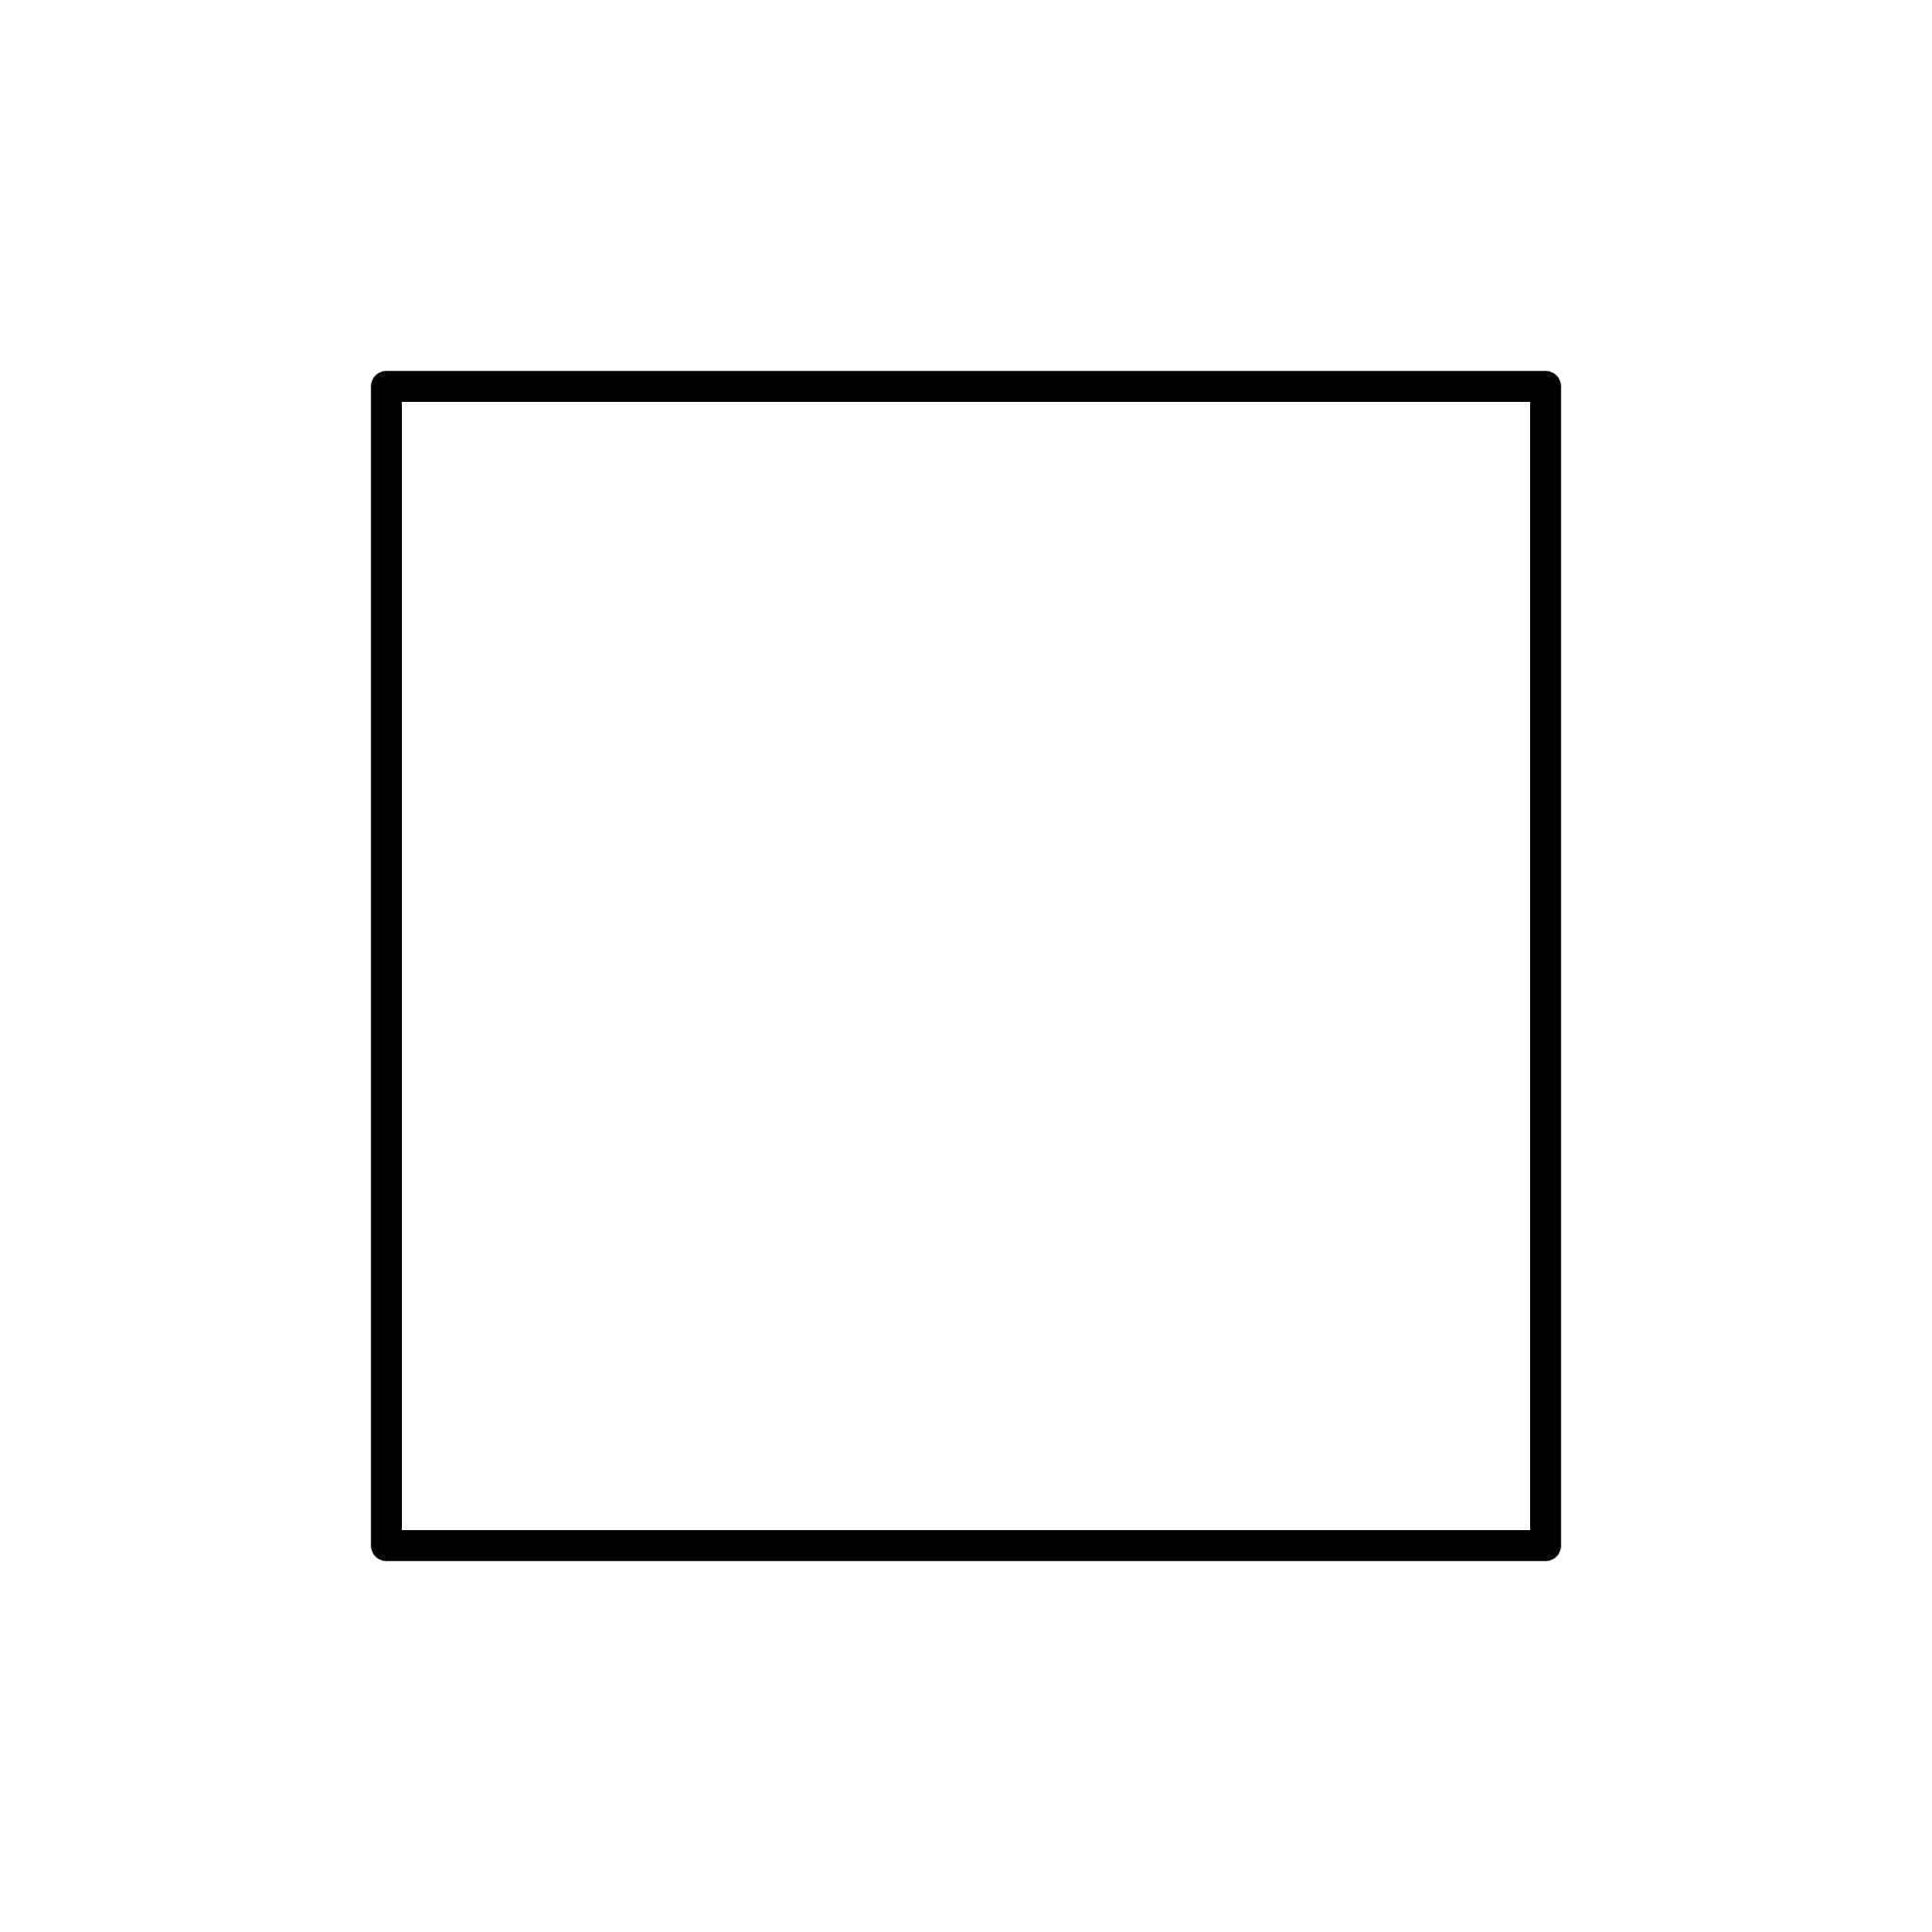
\includegraphics[width=0.25\linewidth]{MichaelImages/Square.png}
		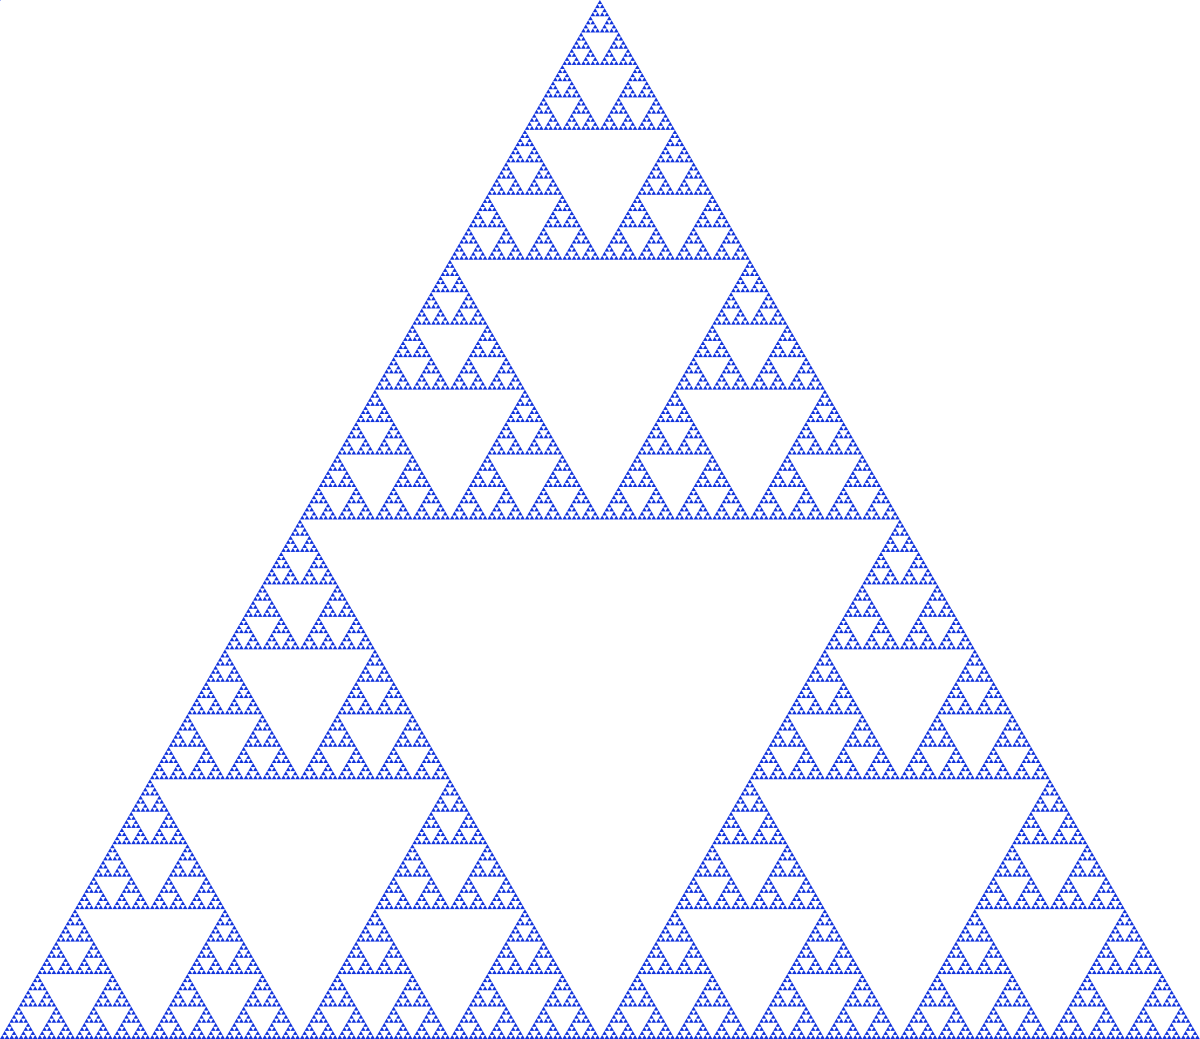
\includegraphics[width=0.25\linewidth]{MichaelImages/Sierpinski_triangle.svg.png}
		\caption{\cite{Sierpinski}}
	\end{figure}
\end{frame}

\begin{frame}{Box-Counting Dimension}
	\begin{itemize}
		\item Place our fractal in grid of "boxes"
		\item How does the number of boxes change as they get smaller?
	\end{itemize}
	
	\begin{center}
		\[N \approx N_0s^{-d} \implies \dim_{box}(S) = \lim_{s \to 0}\frac{log (N(s))}{log(s^{-1})}\] 
	\end{center}
	\begin{figure}
		\centering
		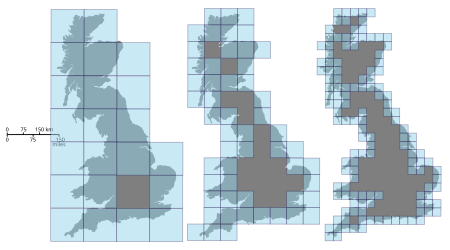
\includegraphics[width=0.25\linewidth]{MichaelImages/Great_Britain_Box.svg.png}
		\caption{Dimension of UK coastline is approx 1.25, (\cite{Mandelbrot1983}, \cite{boxDimensionWiki})}
		\label{fig:enter-label}
	\end{figure}
\end{frame}

\begin{frame}
	\frametitle{Application}
	\begin{itemize}
		\item Medicine
		\begin{itemize}
			\item Identifying tumors in brain MR images \cite{iftekharuddin2003fractal}
			\item Diabetic retinopathy, etc. : blood vessel's diameter \cite{uahabi2015applications}
		\end{itemize}
		\item Economics
		\begin{itemize}
			\item Market properties, price fluctuation, money flow. \cite{takayasu2009fractals}
		\end{itemize}
		\item Geology and Ecology
		\begin{itemize}
			\item Landscape patterns, vegetation structure, animal habitats. \cite{LOEHLE1996271}
		\end{itemize}
		\item Computer science
		\begin{itemize}
			\item Image encryption. \cite{sangavi2019image}
			\item Computer graphics. \cite{sala2021fractal}
		\end{itemize}
		\item Architecture
		\begin{itemize}
			\item Combining aesthetics and functionality. \cite{lorenz2002fractals}
		\end{itemize}
	\end{itemize}
\end{frame}

